\documentclass[11pt,a4paper]{article}

\usepackage[spanish,es-noshorthands]{babel}
\usepackage[T1]{fontenc}
\usepackage[utf8]{inputenc}
\usepackage{lmodern}
\usepackage[a4paper,margin=2.35cm]{geometry}
\usepackage{amsmath}
\usepackage{amssymb}
\usepackage{booktabs}
\usepackage{array}
\usepackage{tabularx}
\usepackage{graphicx}
\usepackage{float}
\usepackage{caption}
\usepackage{enumitem}
\usepackage{xcolor}
\usepackage{hyperref}
\usepackage{xurl}
\usepackage{natbib}

\hypersetup{
    colorlinks=true,
    linkcolor=blue!60!black,
    citecolor=blue!60!black,
    urlcolor=blue!60!black,
    pdftitle={Reporte general final del proyecto TD3 para protesis mioelectrica},
    pdfauthor={Proyecto EMG Prosthesis TD3}
}

\newcolumntype{L}[1]{>{\raggedright\arraybackslash}p{#1}}
\newcolumntype{C}[1]{>{\centering\arraybackslash}p{#1}}
\newcolumntype{Y}{>{\raggedright\arraybackslash}X}

\title{\textbf{Reporte General Final del Proyecto TD3 para una Protesis Mioelectrica}\\
\large Desde la base conceptual hasta la linea residual final sobre \texttt{Agent7250}}
\author{Proyecto \texttt{EMG\_Prosthesis\_TD3}}
\date{26 de marzo de 2026}

\begin{document}
\maketitle

\begin{abstract}
Este documento consolida la linea completa del proyecto de control mioelectrico con TD3, desde su base conceptual inicial hasta el estado final actual. El hilo conductor del reporte es simple: primero hubo que depurar reward, entorno y simulador para obtener un benchmark valido; despues hubo que intentar mejorar ese benchmark sin romper el tracking. La fase previa a la validacion dejo aprendizaje tecnico importante, pero el primer benchmark plenamente defendible aparecio despues del fix del simulador, cuando la corrida de 8000 episodios produjo a \texttt{Agent7250}. A partir de ese punto se abrio una nueva fase, ya no orientada a ``hacer que aprenda'', sino a reducir agresividad y esfuerzo manteniendo el tracking. Se probaron varias lineas de bajo riesgo: continuacion con menor exploracion, exploracion \textit{threshold-aware}, regularizacion de saturacion, \textit{warm-start} offline y una interfaz de accion alineada al actuador. Ninguna reemplazo al benchmark. La intervencion que si aporto una mejora real fue la politica residual sobre \texttt{Agent7250}. El mejor candidato final de esa familia fue \texttt{Agent1850} con \(\alpha_{\mathrm{res}} = 0.20\), cuyo test visual de 50 simulaciones obtuvo \texttt{trackingMSE = 0.043445}, \texttt{trackingMAE = 0.163542}, \texttt{actionL2 = 0.523597}, \texttt{saturationFraction = 0.272637} y \texttt{deltaActionL2 = 0.299262}. Ese resultado cumple \texttt{ConditionB} frente a \texttt{Agent7250} y se toma aqui como punto final operativo del proyecto.
\end{abstract}

\tableofcontents
\newpage

\section{Que documenta este reporte}

Este reporte tiene tres objetivos:
\begin{enumerate}[leftmargin=1.5em]
\item reconstruir la linea del proyecto desde la base conceptual hasta el estado final actual;
\item explicar de forma sencilla por que se tomo cada iniciativa importante;
\item dejar fijado, con criterio tecnico y con evidencia, cual es el mejor agente final de la linea actual.
\end{enumerate}

La idea no es reescribir toda la historia como si todas las corridas hubieran valido igual. Al contrario: una parte importante del trabajo consistio precisamente en aprender a separar:
\begin{itemize}[leftmargin=1.5em]
\item exploracion util,
\item resultados contaminados por problemas del entorno,
\item y benchmark realmente valido.
\end{itemize}

\section{Base conceptual del proyecto}

La raiz conceptual del proyecto es el manuscrito \emph{Continuous Operation of a Myoelectric Hand Prosthesis using the TD3 Reinforcement Learning Algorithm} \citep{fuertes2026continuous}. Ese trabajo fijaba tres ideas que siguieron siendo correctas durante toda la evolucion posterior:
\begin{itemize}[leftmargin=1.5em]
\item el problema es de control continuo sobre cuatro motores;
\item la politica debe mapear observaciones EMG y estado mecanico a acciones continuas;
\item TD3 es una eleccion razonable para ese tipo de tarea \citep{fujimoto2018td3,mathworks_td3_agent,mathworks_td3_options}.
\end{itemize}

Esa base tambien es coherente con la literatura general de control mioelectrico: la protesis no debe responder solo como un clasificador de gestos, sino como un sistema continuo, proporcional y razonablemente suave \citep{chen2023review,done2025prostheticrl}.

\section{Antes del benchmark valido: que hubo que corregir}

\subsection{Reward heredada}

La primera version del repositorio usaba una reward heredada que mezclaba varias ideas a la vez: direccion correcta, castigo por error, incentivos a no quedarse quieto y penalizacion por cambios bruscos. El problema no era que esas ideas fueran absurdas; el problema era que estaban acopladas de forma poco interpretable. En la practica:
\begin{itemize}[leftmargin=1.5em]
\item trataba acciones continuas como si fueran casi discretas;
\item su escala no hacia obvio que termino dominaba realmente;
\item dejaba abierta la puerta a \emph{reward hacking};
\item hacia dificil saber si el agente mejoraba tracking o solo aprendia a explotar huecos de la reward.
\end{itemize}

Ese tipo de problema es bien conocido en \emph{reward shaping}: una reward compleja no necesariamente induce el comportamiento correcto si no esta alineada con el objetivo fisico real \citep{deng2025reward}.

\subsection{Paso a una reward basada en tracking MSE}

Por eso se fue migrando a una reward mucho mas clara:
\[
r_t = -\frac{1}{4}\sum_{i=1}^{4}\left(e_{t,i}^{2} + \lambda_a \tilde{a}_{t,i}^{2} + \lambda_{\Delta a}\left(\tilde{a}_{t,i}-\tilde{a}_{t-1,i}\right)^2\right),
\]
donde el termino dominante es el error de tracking, y los otros dos solo regularizan esfuerzo y brusquedad.

La motivacion fue simple:
\begin{itemize}[leftmargin=1.5em]
\item si el proyecto busca seguimiento continuo, el error de seguimiento debe ser el centro de la reward;
\item si se quiere evitar politicas violentas, eso debe entrar como regularizacion, no como objetivo principal;
\item una formulacion asi es mas compatible con TD3 y mas interpretable durante la auditoria \citep{fujimoto2018td3,lee2024smoothness}.
\end{itemize}

\subsection{Accion efectiva cuantizada}

Otra mejora estructural fue explicitar que la accion realmente aplicada por el entorno no era una variable continua arbitraria, sino una accion efectiva cuantizada en niveles PWM utiles. Esta alineacion era necesaria porque el actor producia valores en \([-1,1]\), pero el simulador y el actuador operaban con bins efectivos.

\subsection{El bug del simulador}

El hallazgo mas importante de toda la historia temprana fue que el simulador estaba roto. La dinamica dependia de \texttt{fit\_C2.mat}, pero el contenido util para mover la protesis estaba vacio, de modo que muchas corridas previas no estaban controlando una planta que realmente se moviera. Ademas, habia un desfase temporal en \texttt{step}.

Consecuencia metodologica:
\begin{itemize}[leftmargin=1.5em]
\item las corridas previas al fix ya no pudieron usarse como benchmark numerico serio;
\item si conservaron valor como etapa de depuracion de reward, logging y estructura del entorno.
\end{itemize}

Este punto es fundamental para entender todo el resto del proyecto: la comparacion valida solo empieza despues del fix del simulador.

\section{Construccion del benchmark valido}

\subsection{Baseline limpio post-fix}

Despues de corregir el simulador, el baseline se estabilizo con:
\begin{itemize}[leftmargin=1.5em]
\item observacion \texttt{markov52},
\item reward \texttt{trackingMseActionRateReward},
\item TD3 feedforward,
\item remapeo efectivo cuantizado,
\item entrenamiento y test en simulacion con dataset pregrabado.
\end{itemize}

La observacion \texttt{markov52} fue una extension razonable del estado base del articulo \citep{fuertes2026continuous}: conserva las features EMG, pero anade informacion mecanica util como delta de encoder y accion previa.

\subsection{De 2000 a 8000 episodios}

La primera corrida post-fix plenamente util fue la de 2000 episodios. Luego se hizo una corrida larga de 8000 episodios y una extension a 12000. El resumen de esos hitos es:

\begin{table}[H]
\centering
\caption{Hitos validos de la linea post-fix antes de la fase residual}
\footnotesize
\setlength{\tabcolsep}{4pt}
\renewcommand{\arraystretch}{1.12}
\begin{tabularx}{\linewidth}{@{}Y C{1.45cm}C{1.45cm}C{1.35cm}C{1.70cm}C{1.55cm}@{}}
\toprule
Agente / etapa & \shortstack{tracking\\MSE} & \shortstack{tracking\\MAE} & \shortstack{action\\L2} & \shortstack{saturation\\Fraction} & \shortstack{deltaAction\\L2} \\
\midrule
2000 episodios\\(nuevo baseline post-fix) & 0.052805 & 0.179093 & 0.674957 & 0.474999 & 0.633264 \\
\texttt{Agent7250}\\en 8000 episodios & 0.043045 & 0.160336 & 0.596444 & 0.392086 & 0.321385 \\
\texttt{Agent11900}\\en 12000 episodios & 0.045189 & 0.164639 & 0.649868 & 0.511786 & 0.305285 \\
\bottomrule
\end{tabularx}
\end{table}

La lectura fue clara:
\begin{itemize}[leftmargin=1.5em]
\item 8000 episodios mejoraron claramente al baseline post-fix inicial;
\item 12000 episodios no superaron el compromiso alcanzado por \texttt{Agent7250};
\item eso indico que el problema ya no era simplemente ``mas episodios''.
\end{itemize}

\begin{figure}[H]
\centering
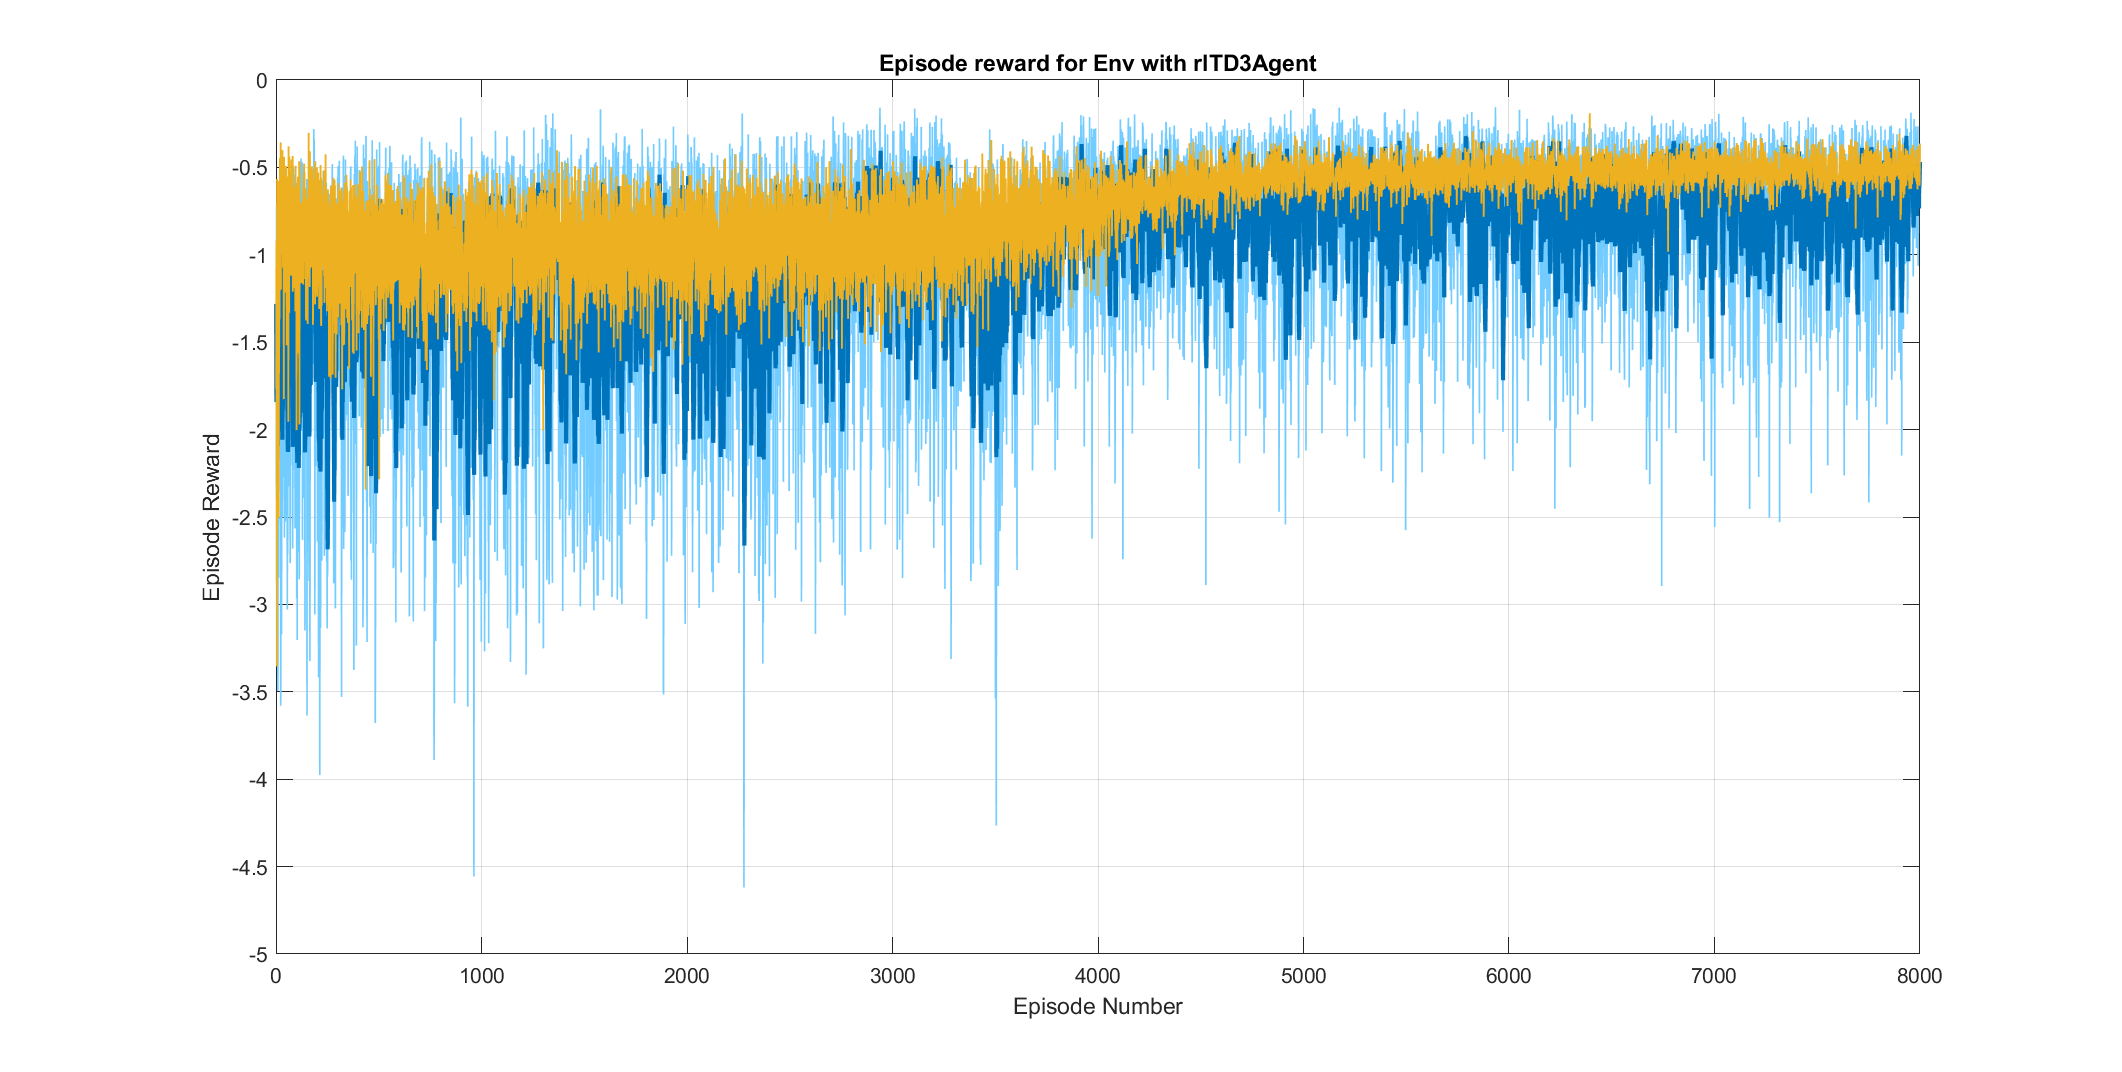
\includegraphics[width=0.92\linewidth]{figures/training_progress_8000eps_valid_baseline.png}
\caption{Progreso de entrenamiento de la corrida valida de 8000 episodios. Esta fue la base del benchmark \texttt{Agent7250}.}
\end{figure}

\begin{figure}[H]
\centering
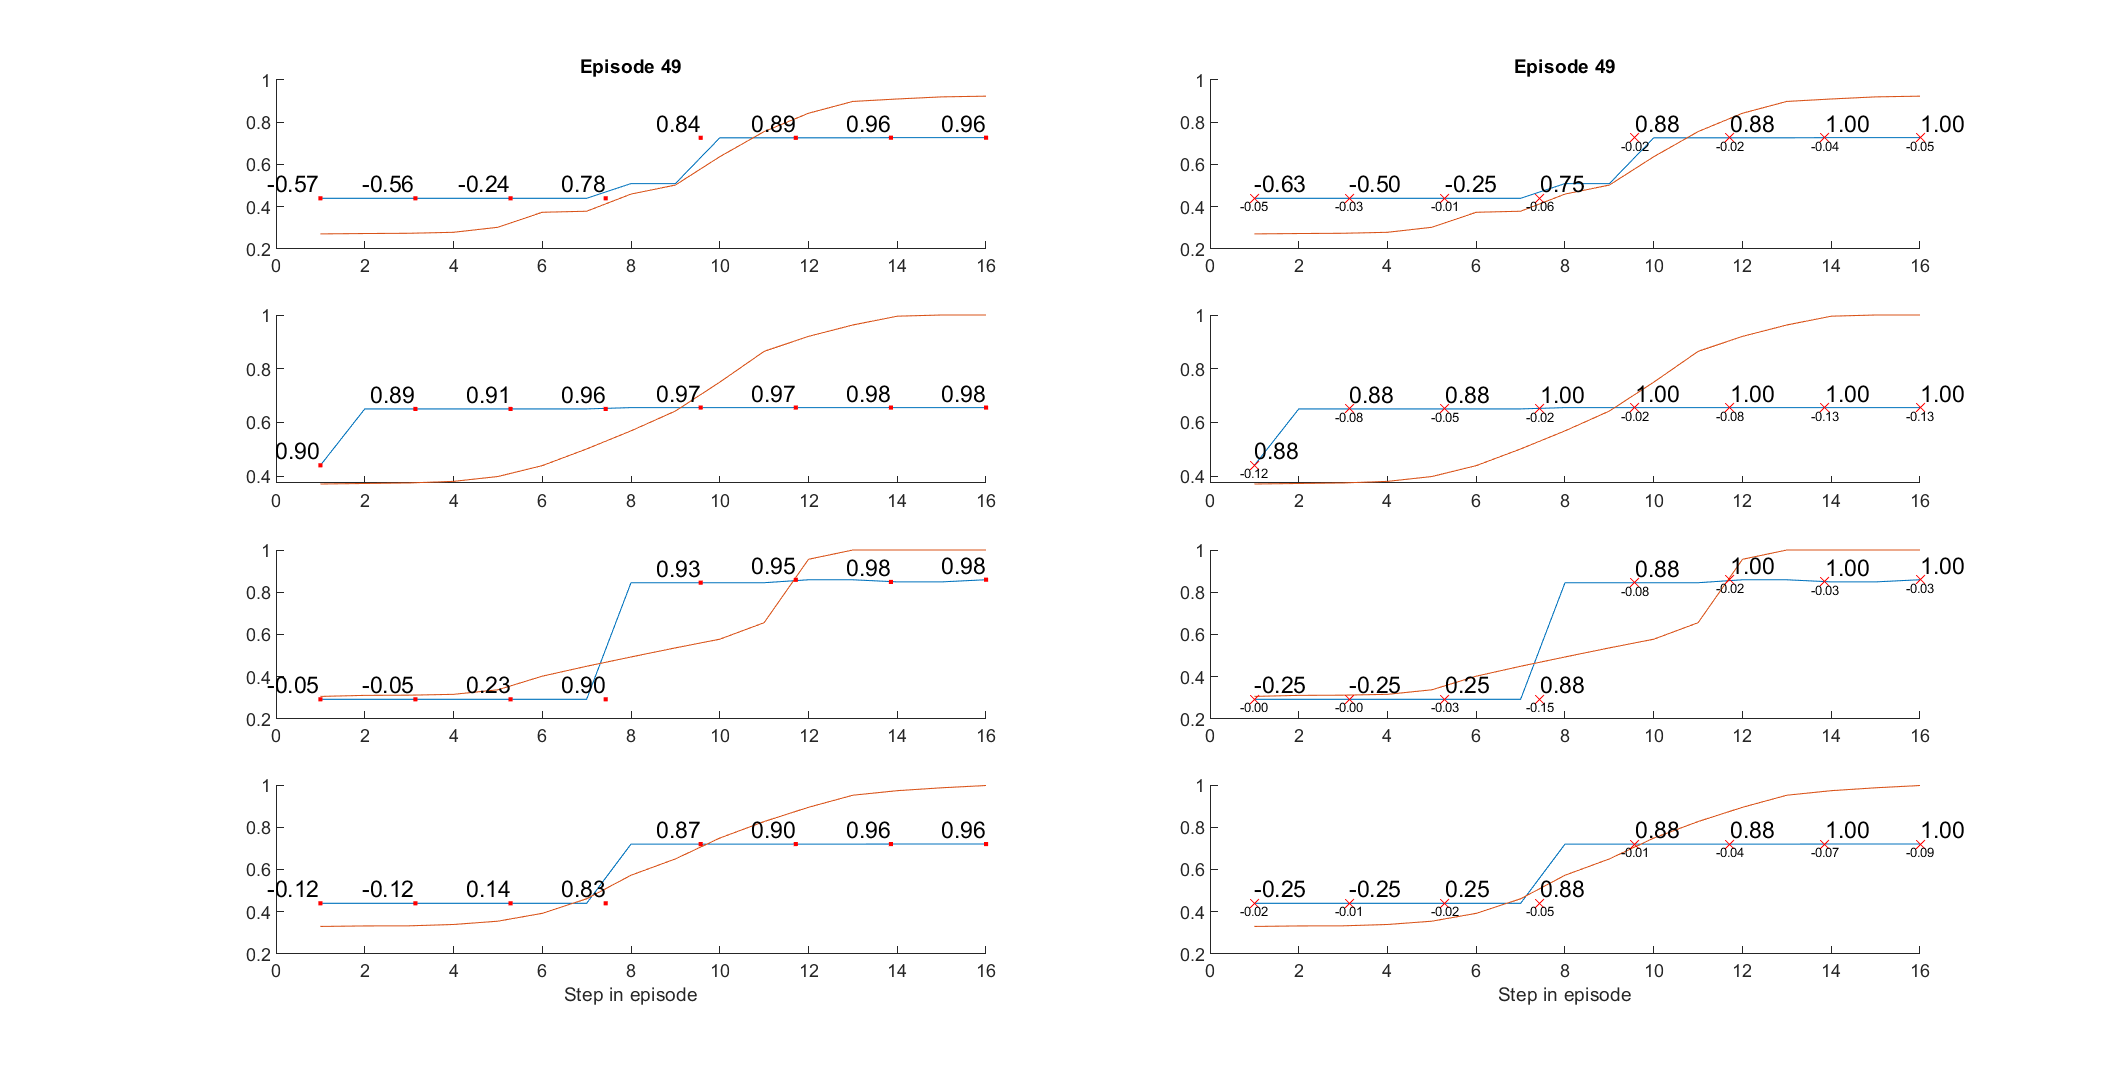
\includegraphics[width=0.90\linewidth]{figures/test_episode_49_valid_baseline_8000.png}
\caption{Ejemplo visual del benchmark \texttt{Agent7250}. El tracking ya es bueno, pero aun aparece una politica relativamente agresiva.}
\end{figure}

\section{Por que fue necesario abrir una fase nueva despues de \texttt{Agent7250}}

Cuando \texttt{Agent7250} quedo fijado como benchmark, el problema ya no era aprender a seguir la referencia desde cero. El problema dominante paso a ser este:

\begin{quote}
mantener o mejorar el tracking sin seguir pagando tanto en saturacion, esfuerzo y agresividad residual.
\end{quote}

Ese cambio de objetivo fue importante, porque reorganizo toda la fase experimental posterior. A partir de ahi ya no se buscaba ``cualquier mejora'', sino una mejora de compromiso.

\section{Experimentos posteriores a \texttt{Agent7250}}

\subsection{Continuacion con menor exploracion}

La primera idea fue continuar \texttt{Agent7250} con menos ruido de exploracion. La razon era simple: si la politica ya estaba en una buena region del espacio de parametros, reducir el ruido podia suavizar el control sin destruir el tracking.

Esa linea produjo un candidato interesante, \texttt{Agent1100}, con:
\begin{itemize}[leftmargin=1.5em]
\item \texttt{trackingMSE = 0.0479},
\item \texttt{actionL2 = 0.5306},
\item \texttt{saturationFraction = 0.3377},
\item \texttt{deltaActionL2 = 0.2752}.
\end{itemize}

La politica fue mas limpia, pero el tracking cayo demasiado. Sirvio como evidencia de que habia margen para suavizar, pero no como reemplazo del benchmark.

\subsection{Exploracion threshold-aware}

Despues se refino esa misma idea alrededor del umbral del actuador. El razonamiento fue repo-especifico: habia una discontinuidad real entre el umbral de activacion y el primer nivel efectivo de PWM. Se penso que un barrido fino alrededor de ese punto podia abrir una mejora nueva.

No ocurrio. Esa ruta confirmo el mejor casi-acierto de la continuacion con menor exploracion, pero no produjo un agente nuevo superior.

\subsection{Regularizacion por saturacion}

Tambien se probo una reward con penalizacion explicita de saturacion. Esa idea estaba bien motivada por el problema observado: si la politica saturaba demasiado, parecia razonable castigar explicitamente la cercania al borde del actuador.

El problema fue que esa reward empujo al sistema hacia politicas demasiado timidas. El tracking empeoro mucho aunque bajaran esfuerzo y saturacion. La linea fue metodologicamente util, pero quedo cerrada como resultado negativo.

\subsection{Warm-start offline}

Otra ruta fue crear un agente nuevo con una fase offline de \textit{warm-start}. La motivacion era introducir un prior de control mas suave antes del entrenamiento online.

De nuevo, la politica resultante quedo demasiado conservadora. La experiencia fue util para confirmar que el proyecto no necesitaba tanto ``inventar otra politica'', sino encontrar una forma mas segura de corregir una politica ya fuerte.

\subsection{Interfaz de accion alineada al actuador}

Tambien se probo una deformacion continua de la accion antes del remapeo final, buscando alinear mejor la salida del actor con los bins fisicamente utiles del actuador. La idea era razonable porque el repo si tiene una discontinuidad real entre accion continua y accion efectiva.

El resultado fue el contrario al deseado: la politica exploto esa alineacion de forma agresiva y colapso a bins altos. Mejoro algo de tracking en algunos checkpoints, pero a costa de mucho mas borde y mucho mas esfuerzo.

\subsection{Resumen comparativo}

\begin{table}[H]
\centering
\caption{Lectura corta de las intervenciones posteriores a \texttt{Agent7250}}
\begin{tabularx}{\linewidth}{L{3.4cm}Y Y}
\toprule
Intervencion & Por que se intento & Resultado \\
\midrule
Baja exploracion & Suavizar una politica ya buena sin cambiar reward ni arquitectura & Mejoro suavidad, pero perdio demasiado tracking. \\
Threshold-aware & Explotar la discontinuidad real del actuador de forma mas fina & No mejoro el casi-acierto previo. \\
Reward de saturacion & Atacar de forma directa la tendencia a saturar & Sobre-regularizo y genero politicas demasiado timidas. \\
Warm-start offline & Introducir un prior suave antes del online RL & Muy conservador; no supero el benchmark. \\
Interfaz de accion alineada & Reducir el hueco entre accion continua y accion efectiva & Demasiado agresiva; empujo mucho al borde. \\
Residual TD3 & Corregir una politica buena sin reemplazarla por completo & Primera mejora aceptable y defendible. \\
\bottomrule
\end{tabularx}
\end{table}

\begin{figure}[H]
\centering
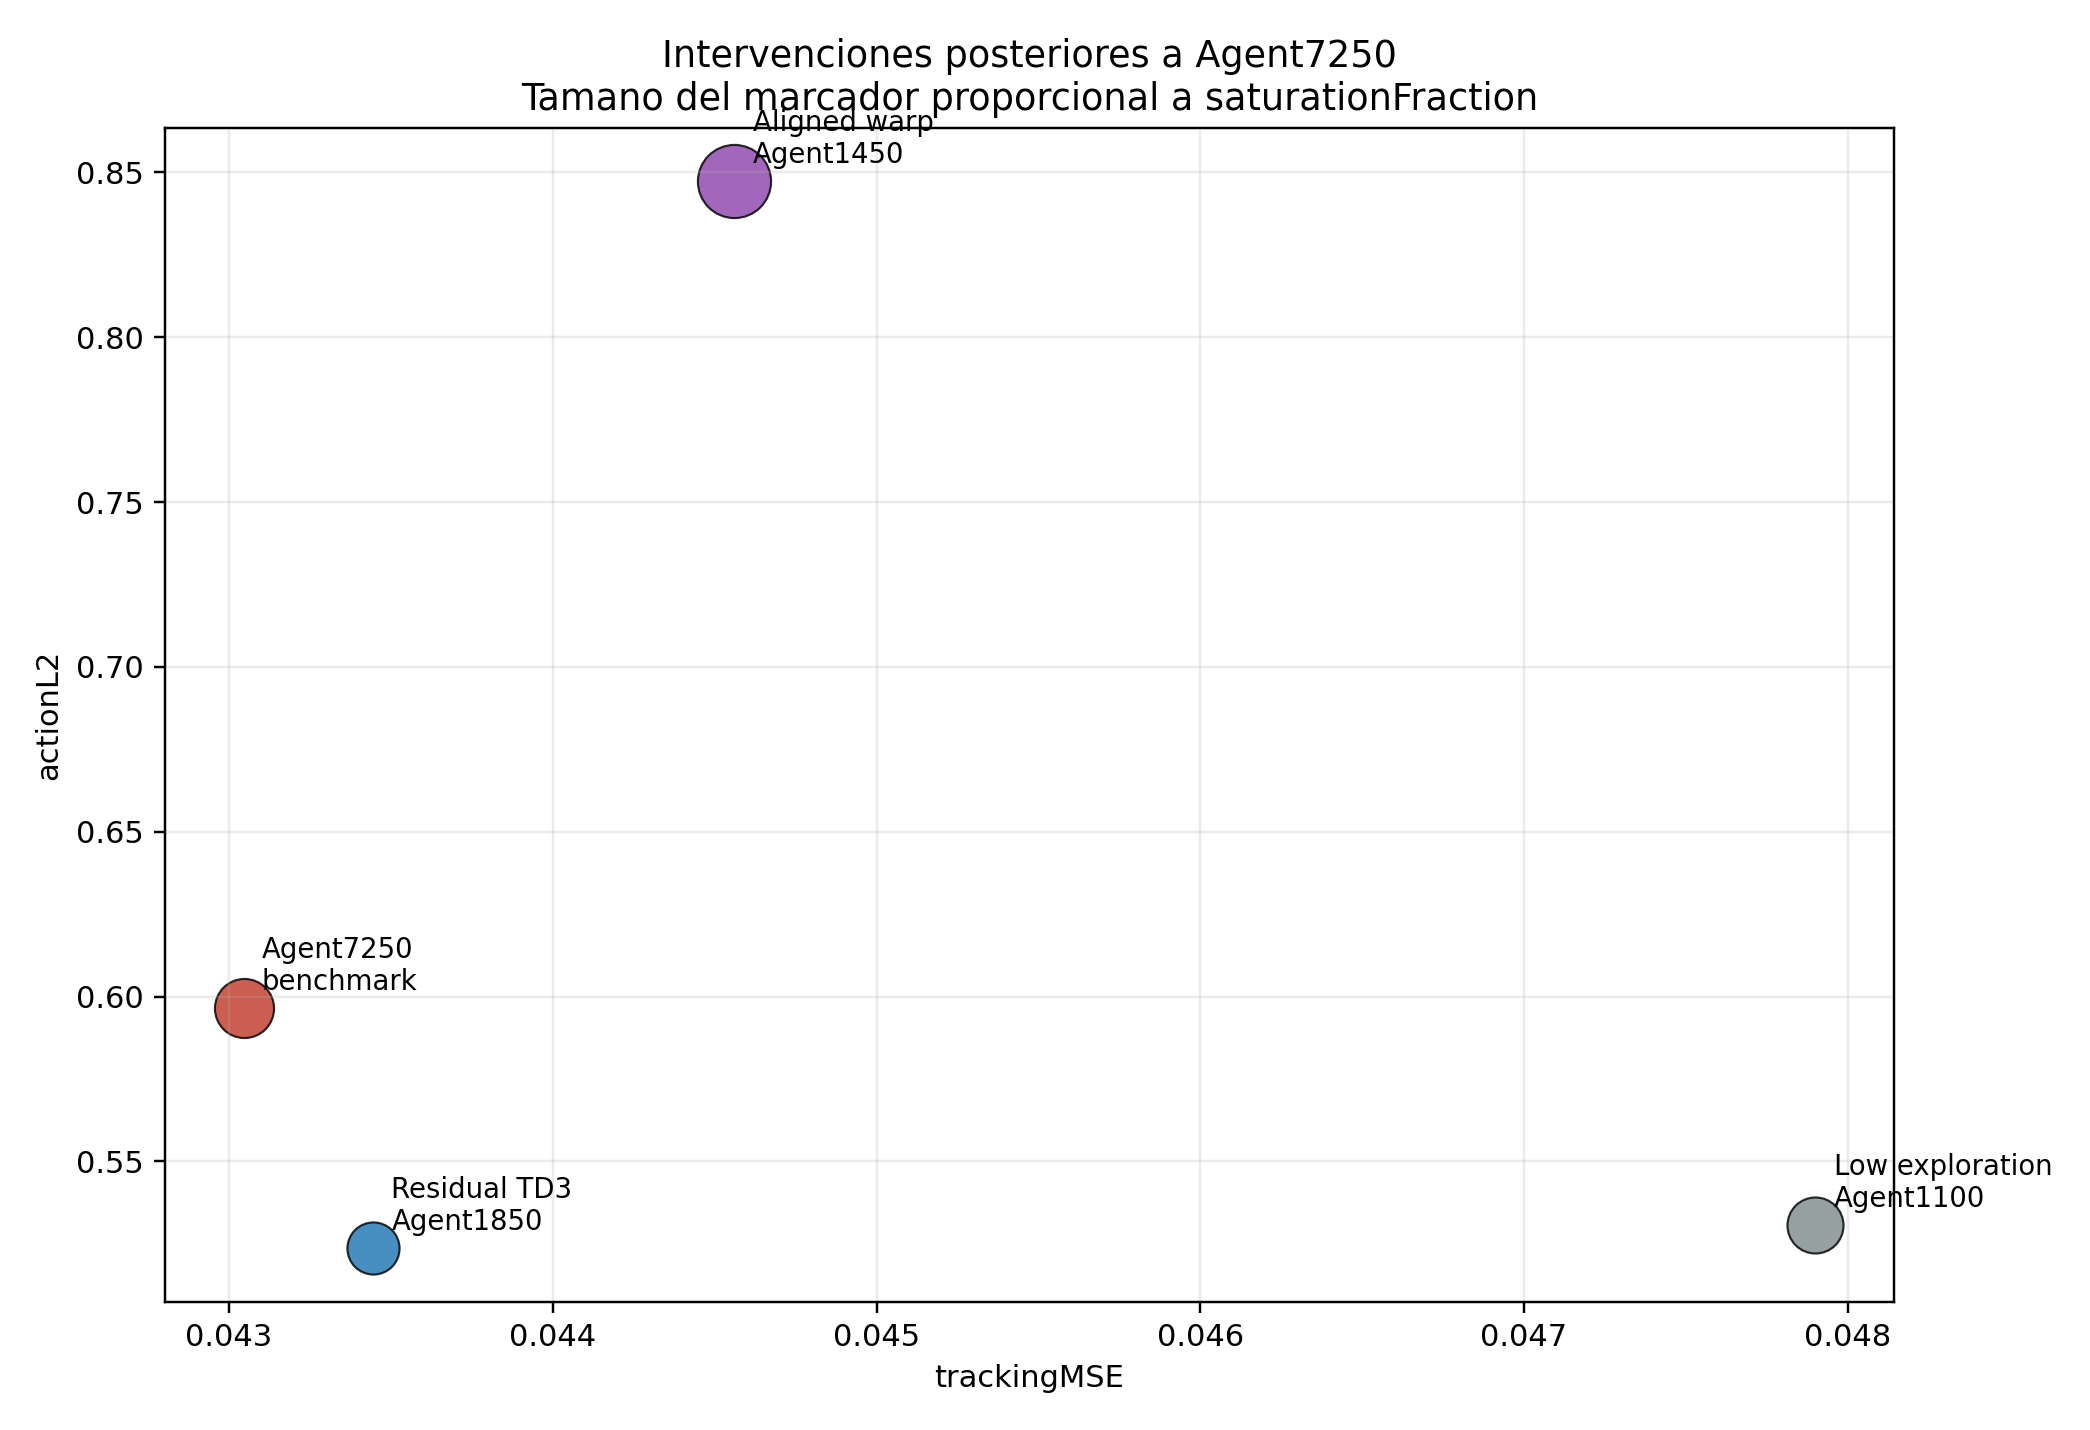
\includegraphics[width=0.92\linewidth]{figures/post7250_interventions_tradeoff_20260326.png}
\caption{Intervenciones clave posteriores a \texttt{Agent7250}. La linea residual es la unica que mejora el compromiso global sin colapsar a un extremo.}
\end{figure}

\section{La fase nueva que si funciono: Residual TD3}

\subsection{Por que la idea residual tenia sentido}

La intuicion de la fase residual fue distinta a la de las lineas anteriores. En vez de seguir moviendo toda la politica, se mantuvo congelada la politica base \texttt{Agent7250} y se aprendio solo una correccion pequena por estado. Esa idea esta alineada con \emph{Residual Policy Learning}: cuando ya existe un controlador razonable, a menudo conviene aprender solo el termino faltante \citep{silver2018residual,schaff2020shared,resfit2025}.

Aplicado a este proyecto, el razonamiento fue:
\begin{itemize}[leftmargin=1.5em]
\item \texttt{Agent7250} ya resolvia bien el tracking;
\item los intentos de mover toda la politica terminaban en un extremo o en otro;
\item era mas sensato aprender una correccion pequena alrededor de una base fuerte.
\end{itemize}

\subsection{Que se implemento}

La politica residual se definio como:
\[
a(s) = \mathrm{clip}\Big(a_{\mathrm{base}}(s) + \alpha_{\mathrm{res}}\,a_{\mathrm{res}}(s,a_{\mathrm{base}}), -1, 1\Big),
\]
donde:
\begin{itemize}[leftmargin=1.5em]
\item \(a_{\mathrm{base}}\) es la accion del actor congelado de \texttt{Agent7250};
\item \(a_{\mathrm{res}}\) es la correccion aprendible;
\item \(\alpha_{\mathrm{res}}\) controla cuanto puede apartarse la politica final respecto a la base.
\end{itemize}

La implementacion se monto dentro del propio actor residual, no en el entorno, para que el critico vea la accion final real. MATLAB y su API de actores deterministas y \texttt{dlnetwork} hacian viable esta estrategia \citep{mathworks_continuous_actor,mathworks_function_layer}.

\subsection{Piloto residual principal}

El piloto principal uso:
\begin{itemize}[leftmargin=1.5em]
\item base checkpoint: \texttt{Agent7250},
\item \(\alpha_{\mathrm{res}} = 0.20\),
\item exploracion reducida \texttt{0.02 / 0.002 / 1e-4},
\item \texttt{2000} episodios.
\end{itemize}

Su mejor checkpoint auditado fue \texttt{Agent1850}, y el test visual de 50 simulaciones dio:

\begin{table}[H]
\centering
\caption{Benchmark vs mejor residual del piloto}
\begin{tabular}{lrr}
\toprule
Metrica & \texttt{Agent7250} & Residual \texttt{Agent1850} \\
\midrule
\texttt{trackingMSE} & 0.043045 & 0.043445 \\
\texttt{trackingMAE} & 0.160336 & 0.163542 \\
\texttt{actionL2} & 0.596444 & 0.523597 \\
\texttt{saturationFraction} & 0.392086 & 0.272637 \\
\texttt{deltaActionL2} & 0.321385 & 0.299262 \\
\bottomrule
\end{tabular}
\end{table}

Ese resultado fue el primer avance serio de toda la fase posterior al benchmark. El tracking empeoro menos de un \(1\%\), mientras que esfuerzo y saturacion bajaron con claridad. Bajo la regla del proyecto, el candidato quedo como \texttt{ConditionB}.

\begin{figure}[H]
\centering
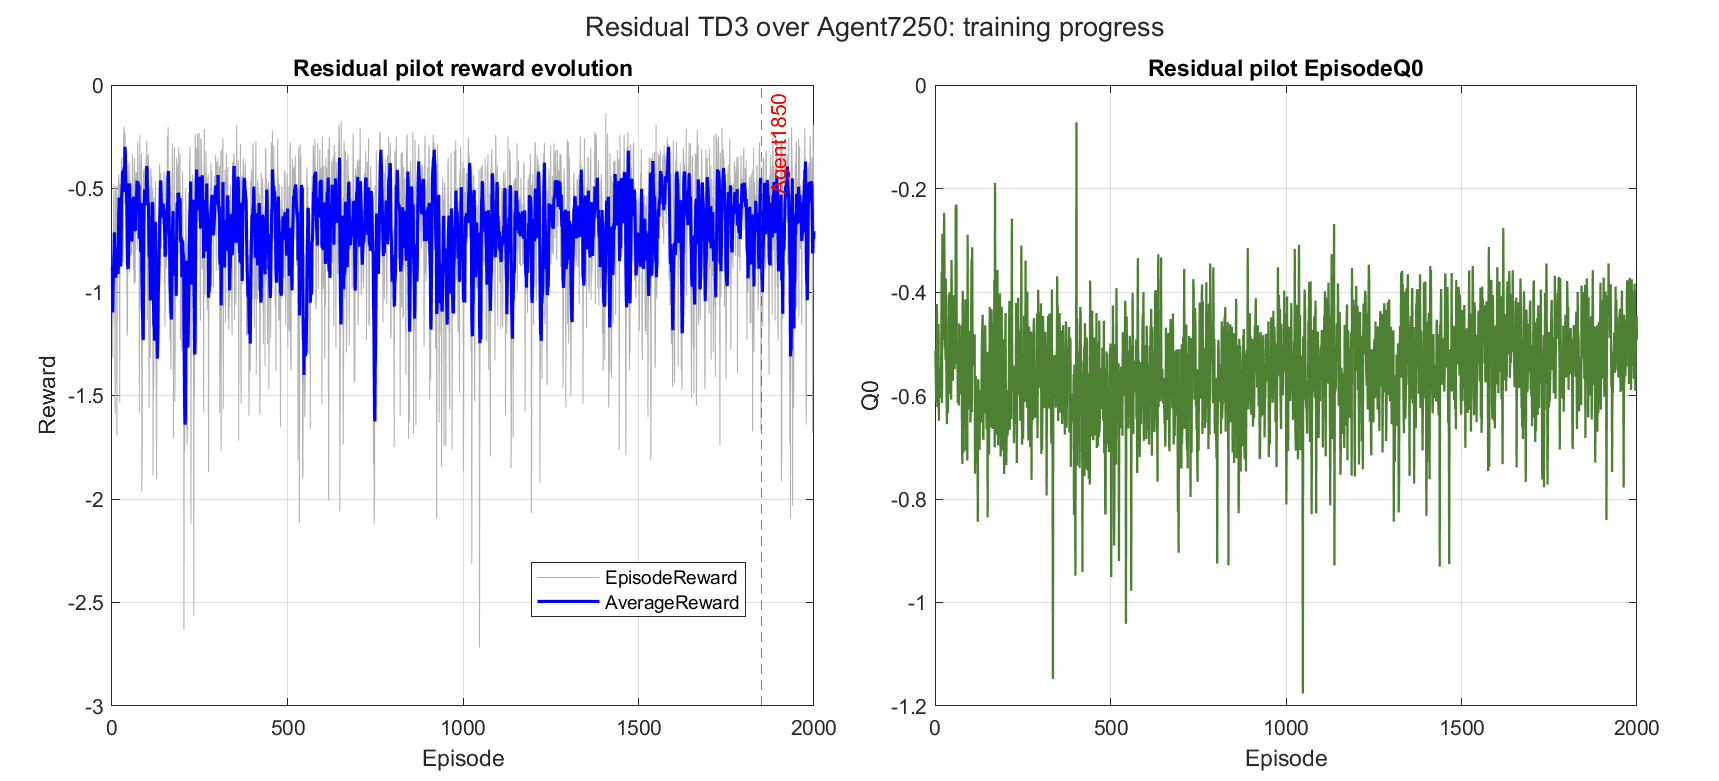
\includegraphics[width=0.92\linewidth]{figures/residual_agent1850_training_progress_20260326.png}
\caption{Evolucion de reward y \texttt{EpisodeQ0} del piloto residual principal. El mejor checkpoint real no se selecciono por reward final, sino por auditoria y test.}
\end{figure}

\begin{figure}[H]
\centering
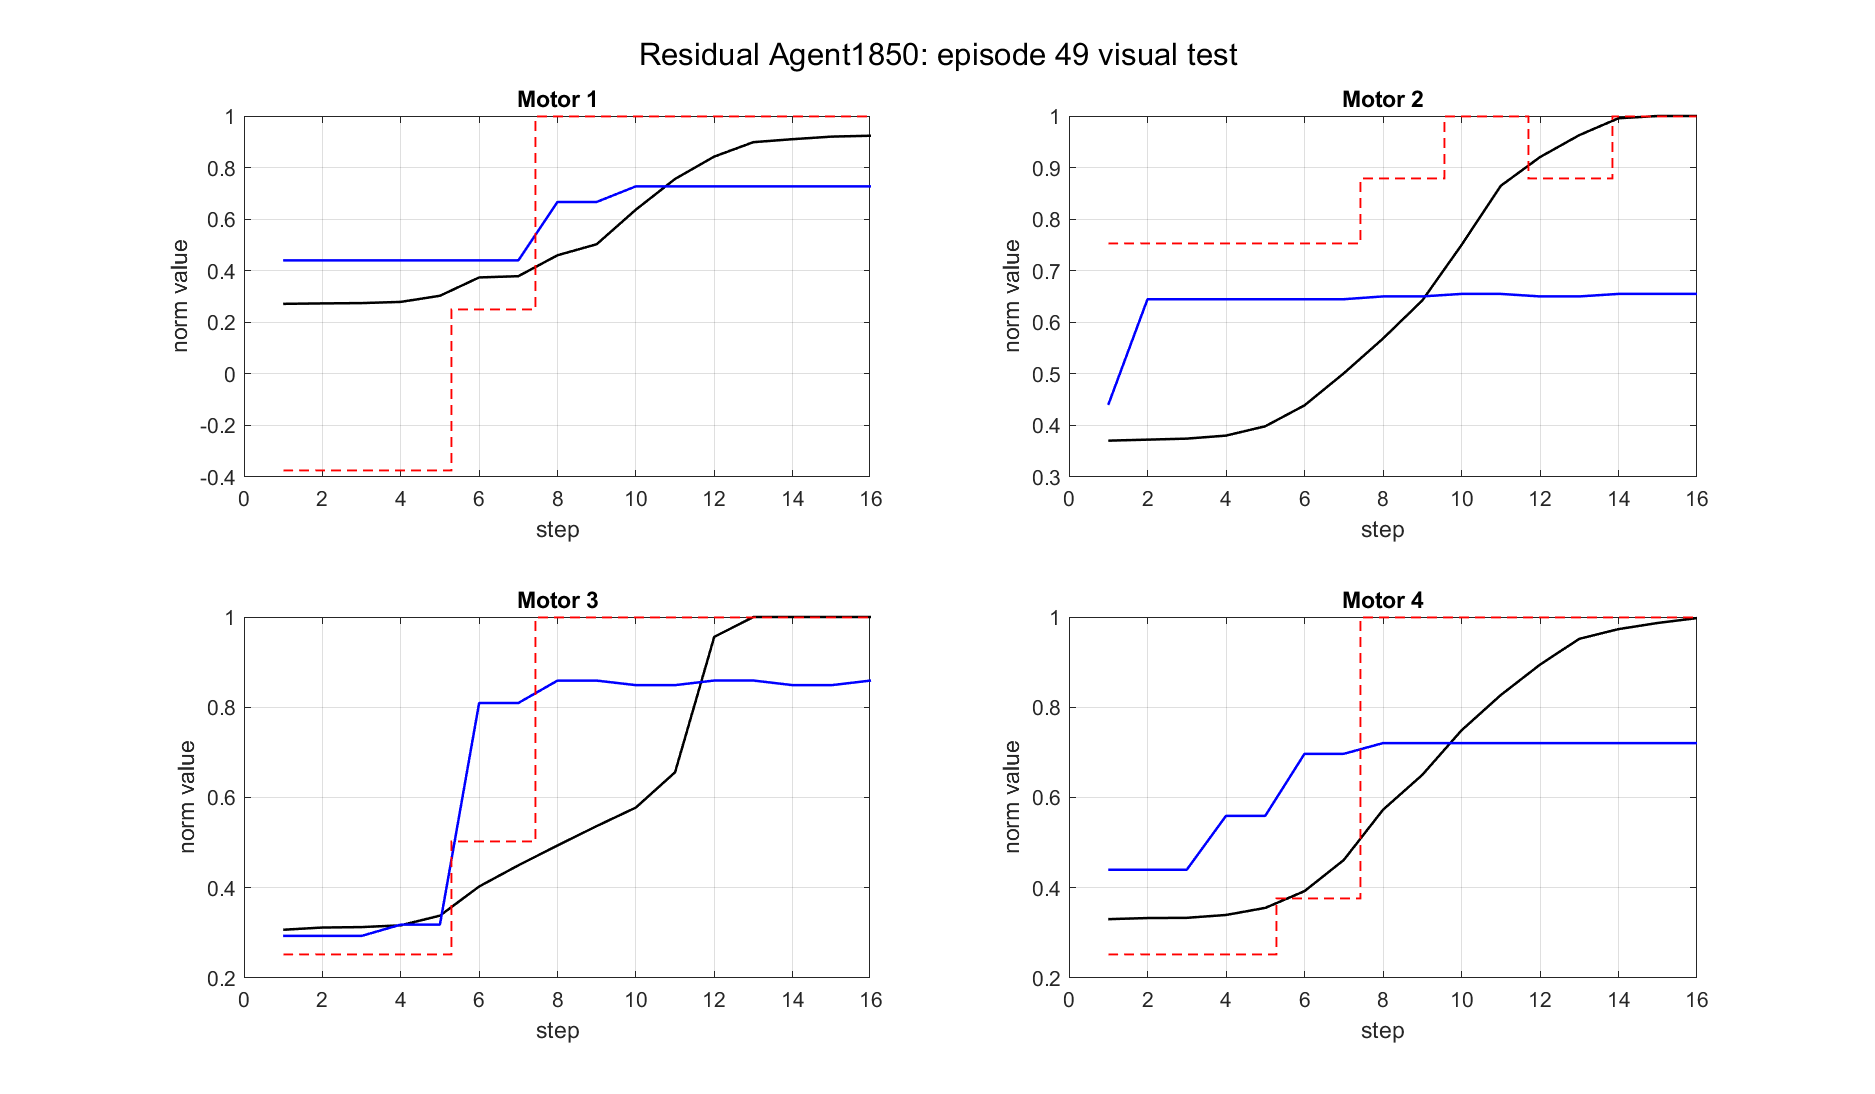
\includegraphics[width=0.92\linewidth]{figures/residual_agent1850_episode49_20260326.png}
\caption{Ejemplo del test visual del residual \texttt{Agent1850}. Se observa un seguimiento cercano al benchmark con una accion efectiva mas contenida.}
\end{figure}

\subsection{Por que no se eligio ``mas episodios''}

Despues del piloto se corrio una extension mas fuerte desde el residual bueno. La hipotesis era razonable: si el mejor checkpoint habia aparecido tarde, tal vez habia margen de mejora con mas entrenamiento.

No ocurrio. La extension no mejoro el compromiso global. La mejor politica de esa continuacion salio peor que el residual original en tracking y esfuerzo. Eso cerro la idea de ``seguir entrenando igual'' como explotacion principal.

\subsection{Que es alpha\_res y por que hubo barridos}

Una vez demostrado que la idea residual funcionaba, la pregunta correcta ya no era si usar residual o no, sino cual debia ser el tamano de la correccion residual. Ese papel lo cumple \(\alpha_{\mathrm{res}}\):
\begin{itemize}[leftmargin=1.5em]
\item si \(\alpha_{\mathrm{res}}\) es muy pequeno, la residual no tiene fuerza suficiente para corregir a la base;
\item si es muy grande, la politica final deja de comportarse como una correccion y vuelve a arriesgar agresividad excesiva;
\item el mejor valor debe quedar entre esos dos extremos.
\end{itemize}

Por eso hubo dos barridos:
\begin{enumerate}[leftmargin=1.5em]
\item un sweep corto: \(\{0.10, 0.20, 0.30\}\);
\item un refinamiento fino: \(\{0.18, 0.20, 0.22, 0.25\}\).
\end{enumerate}

\subsection{Resultado de los barridos}

\begin{table}[H]
\centering
\caption{Resultado consolidado de los barridos de alpha\_res}
\begin{tabular}{lrrrrl}
\toprule
alpha\_res & trackingMSE & actionL2 & saturationFraction & deltaActionL2 & Estado final \\
\midrule
0.10 & 0.042506 & 0.643112 & 0.498572 & 0.263525 & Rejected \\
0.18 & 0.044189 & 0.665430 & 0.482118 & 0.274781 & Rejected \\
0.20 & 0.043445 & 0.523597 & 0.272637 & 0.299262 & ConditionB \\
0.22 & 0.043566 & 0.602889 & 0.378192 & 0.276052 & Rejected \\
0.25 & 0.042503 & 0.625515 & 0.451917 & 0.258078 & Rejected \\
0.30 & 0.044501 & 0.533454 & 0.301742 & 0.325751 & Rejected \\
\bottomrule
\end{tabular}
\end{table}

La conclusion fue robusta:
\begin{itemize}[leftmargin=1.5em]
\item \(\alpha = 0.20\) no solo fue el mejor del piloto; sobrevivio tambien al sweep corto y al refinamiento fino;
\item \(\alpha = 0.10\) fue demasiado debil;
\item \(\alpha = 0.30\) y la zona alta tendieron a sobrecorregir;
\item la zona fina alrededor de \(0.20\) tampoco produjo un punto mejor.
\end{itemize}

\begin{figure}[H]
\centering
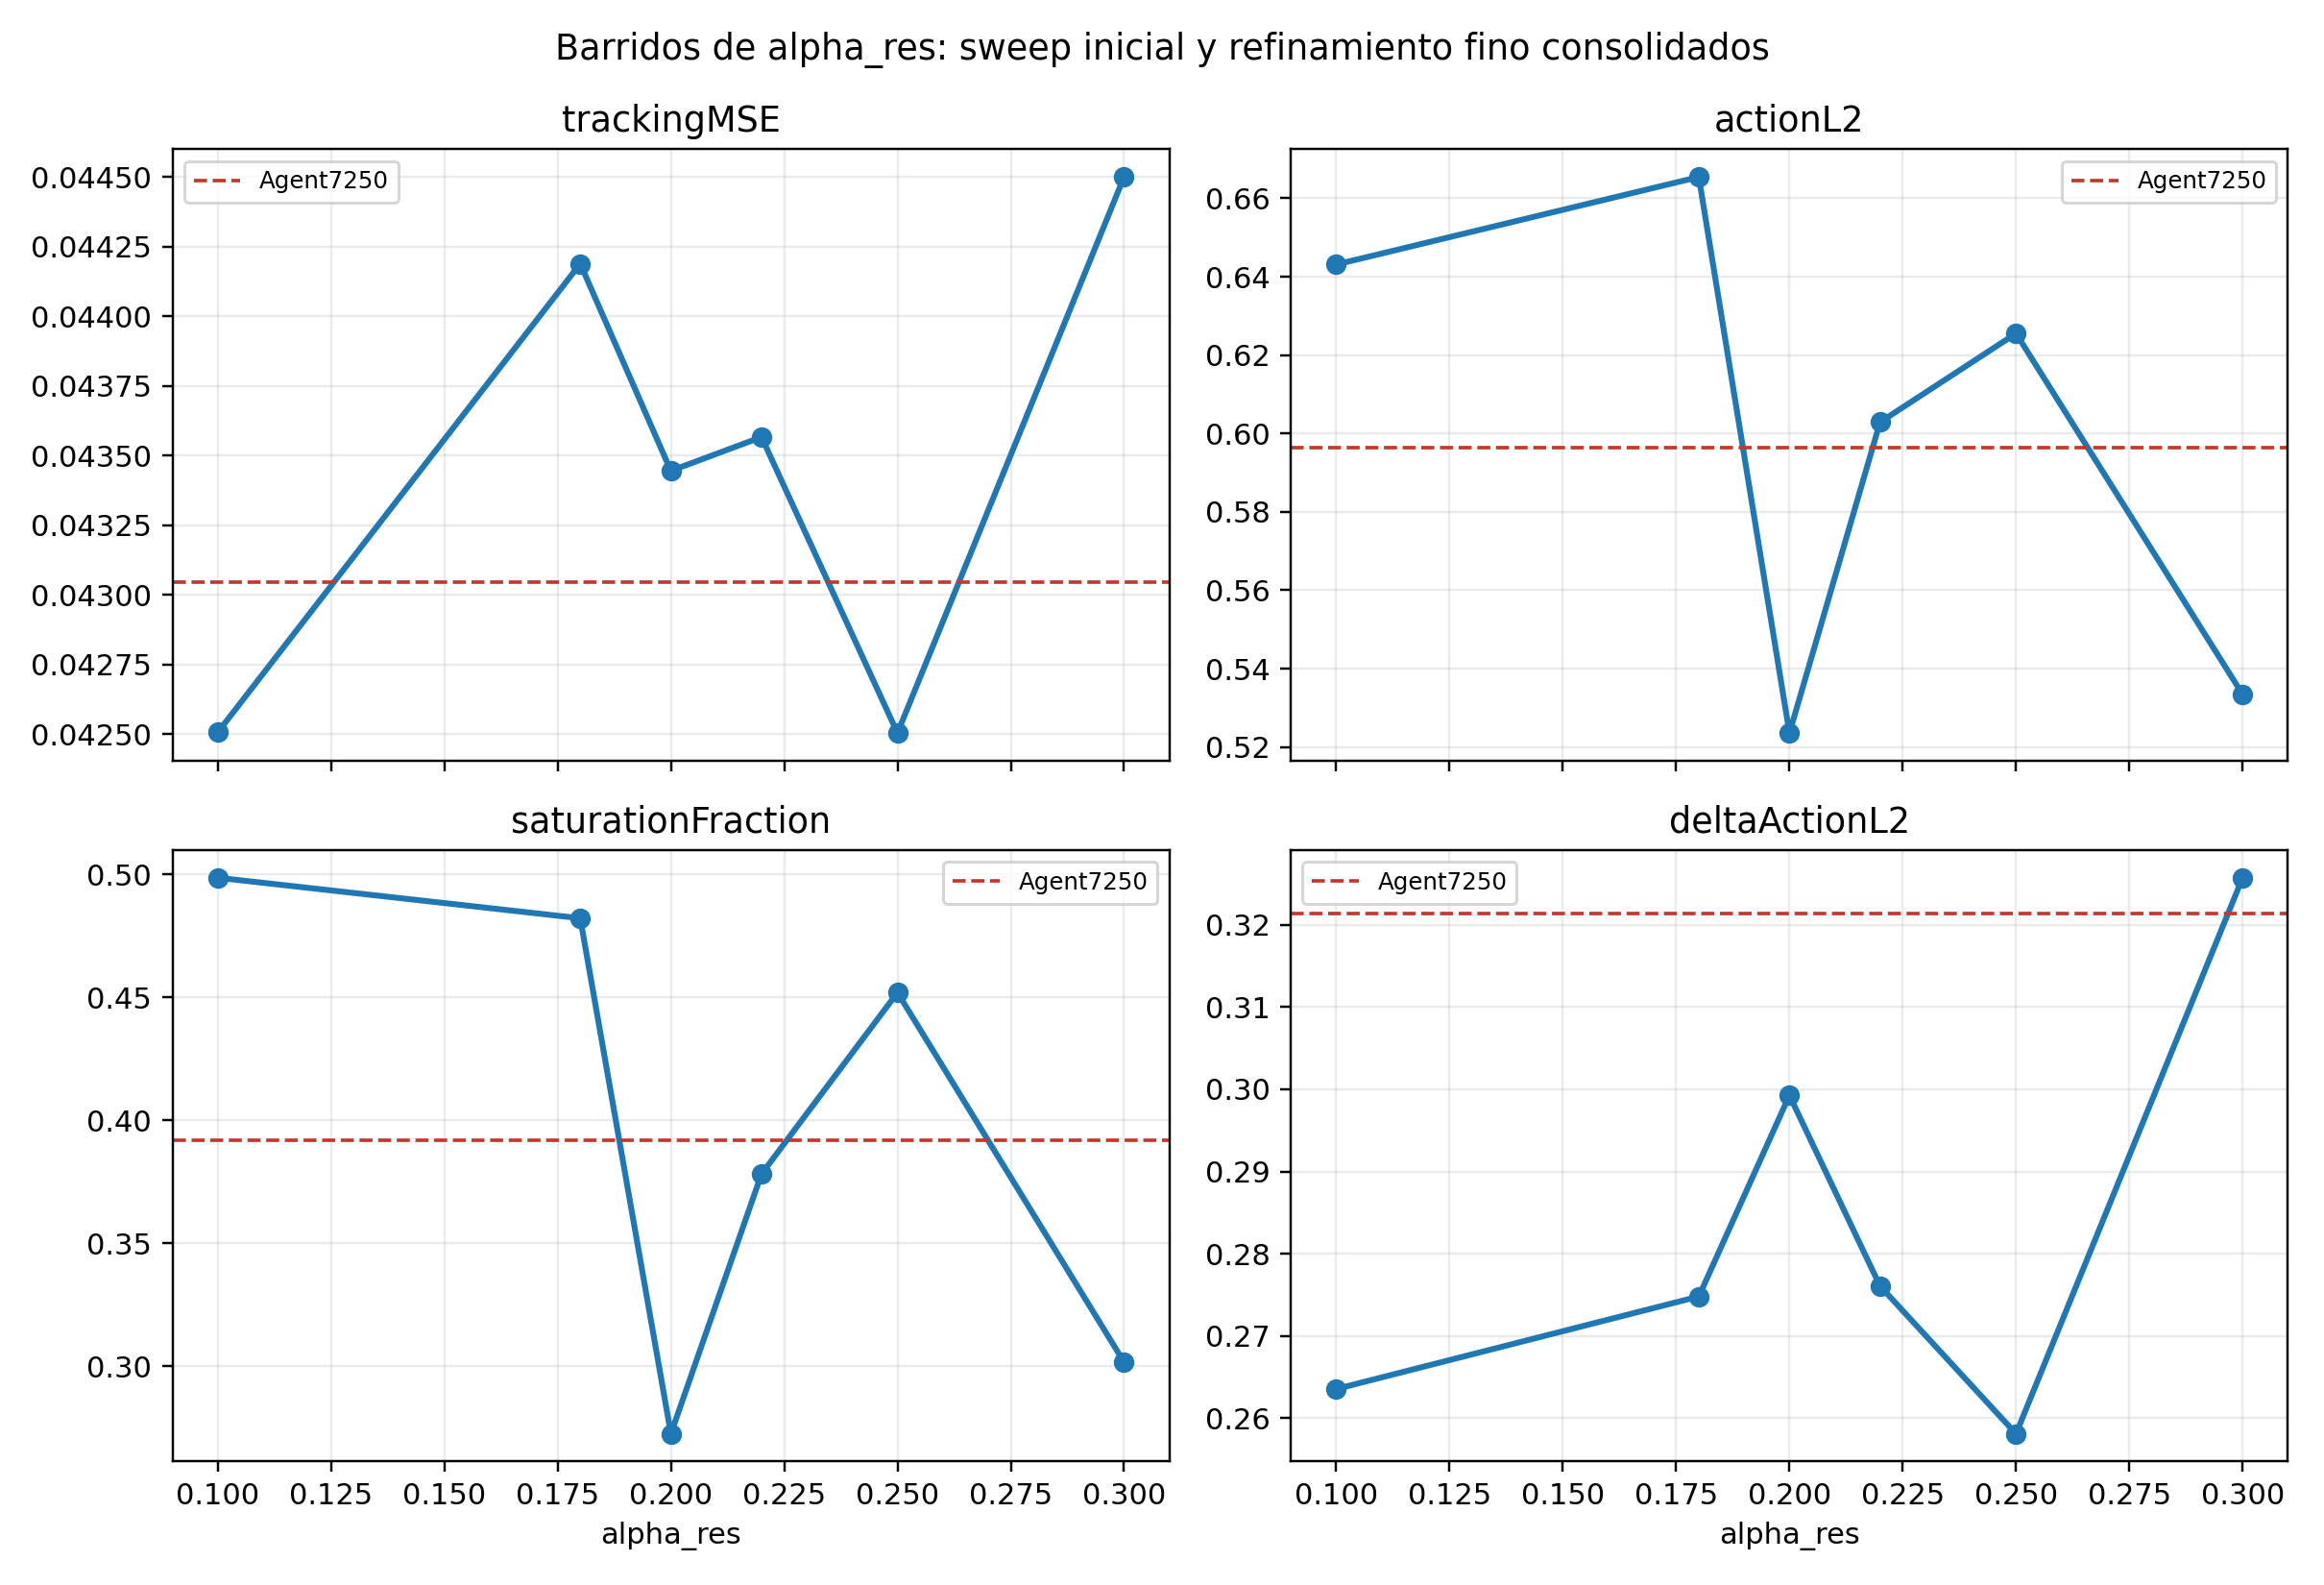
\includegraphics[width=0.98\linewidth]{figures/residual_alpha_sweep_metrics_20260326.png}
\caption{Metricas finales de los barridos de alpha\_res. El benchmark \texttt{Agent7250} aparece como referencia horizontal.}
\end{figure}

\begin{figure}[H]
\centering
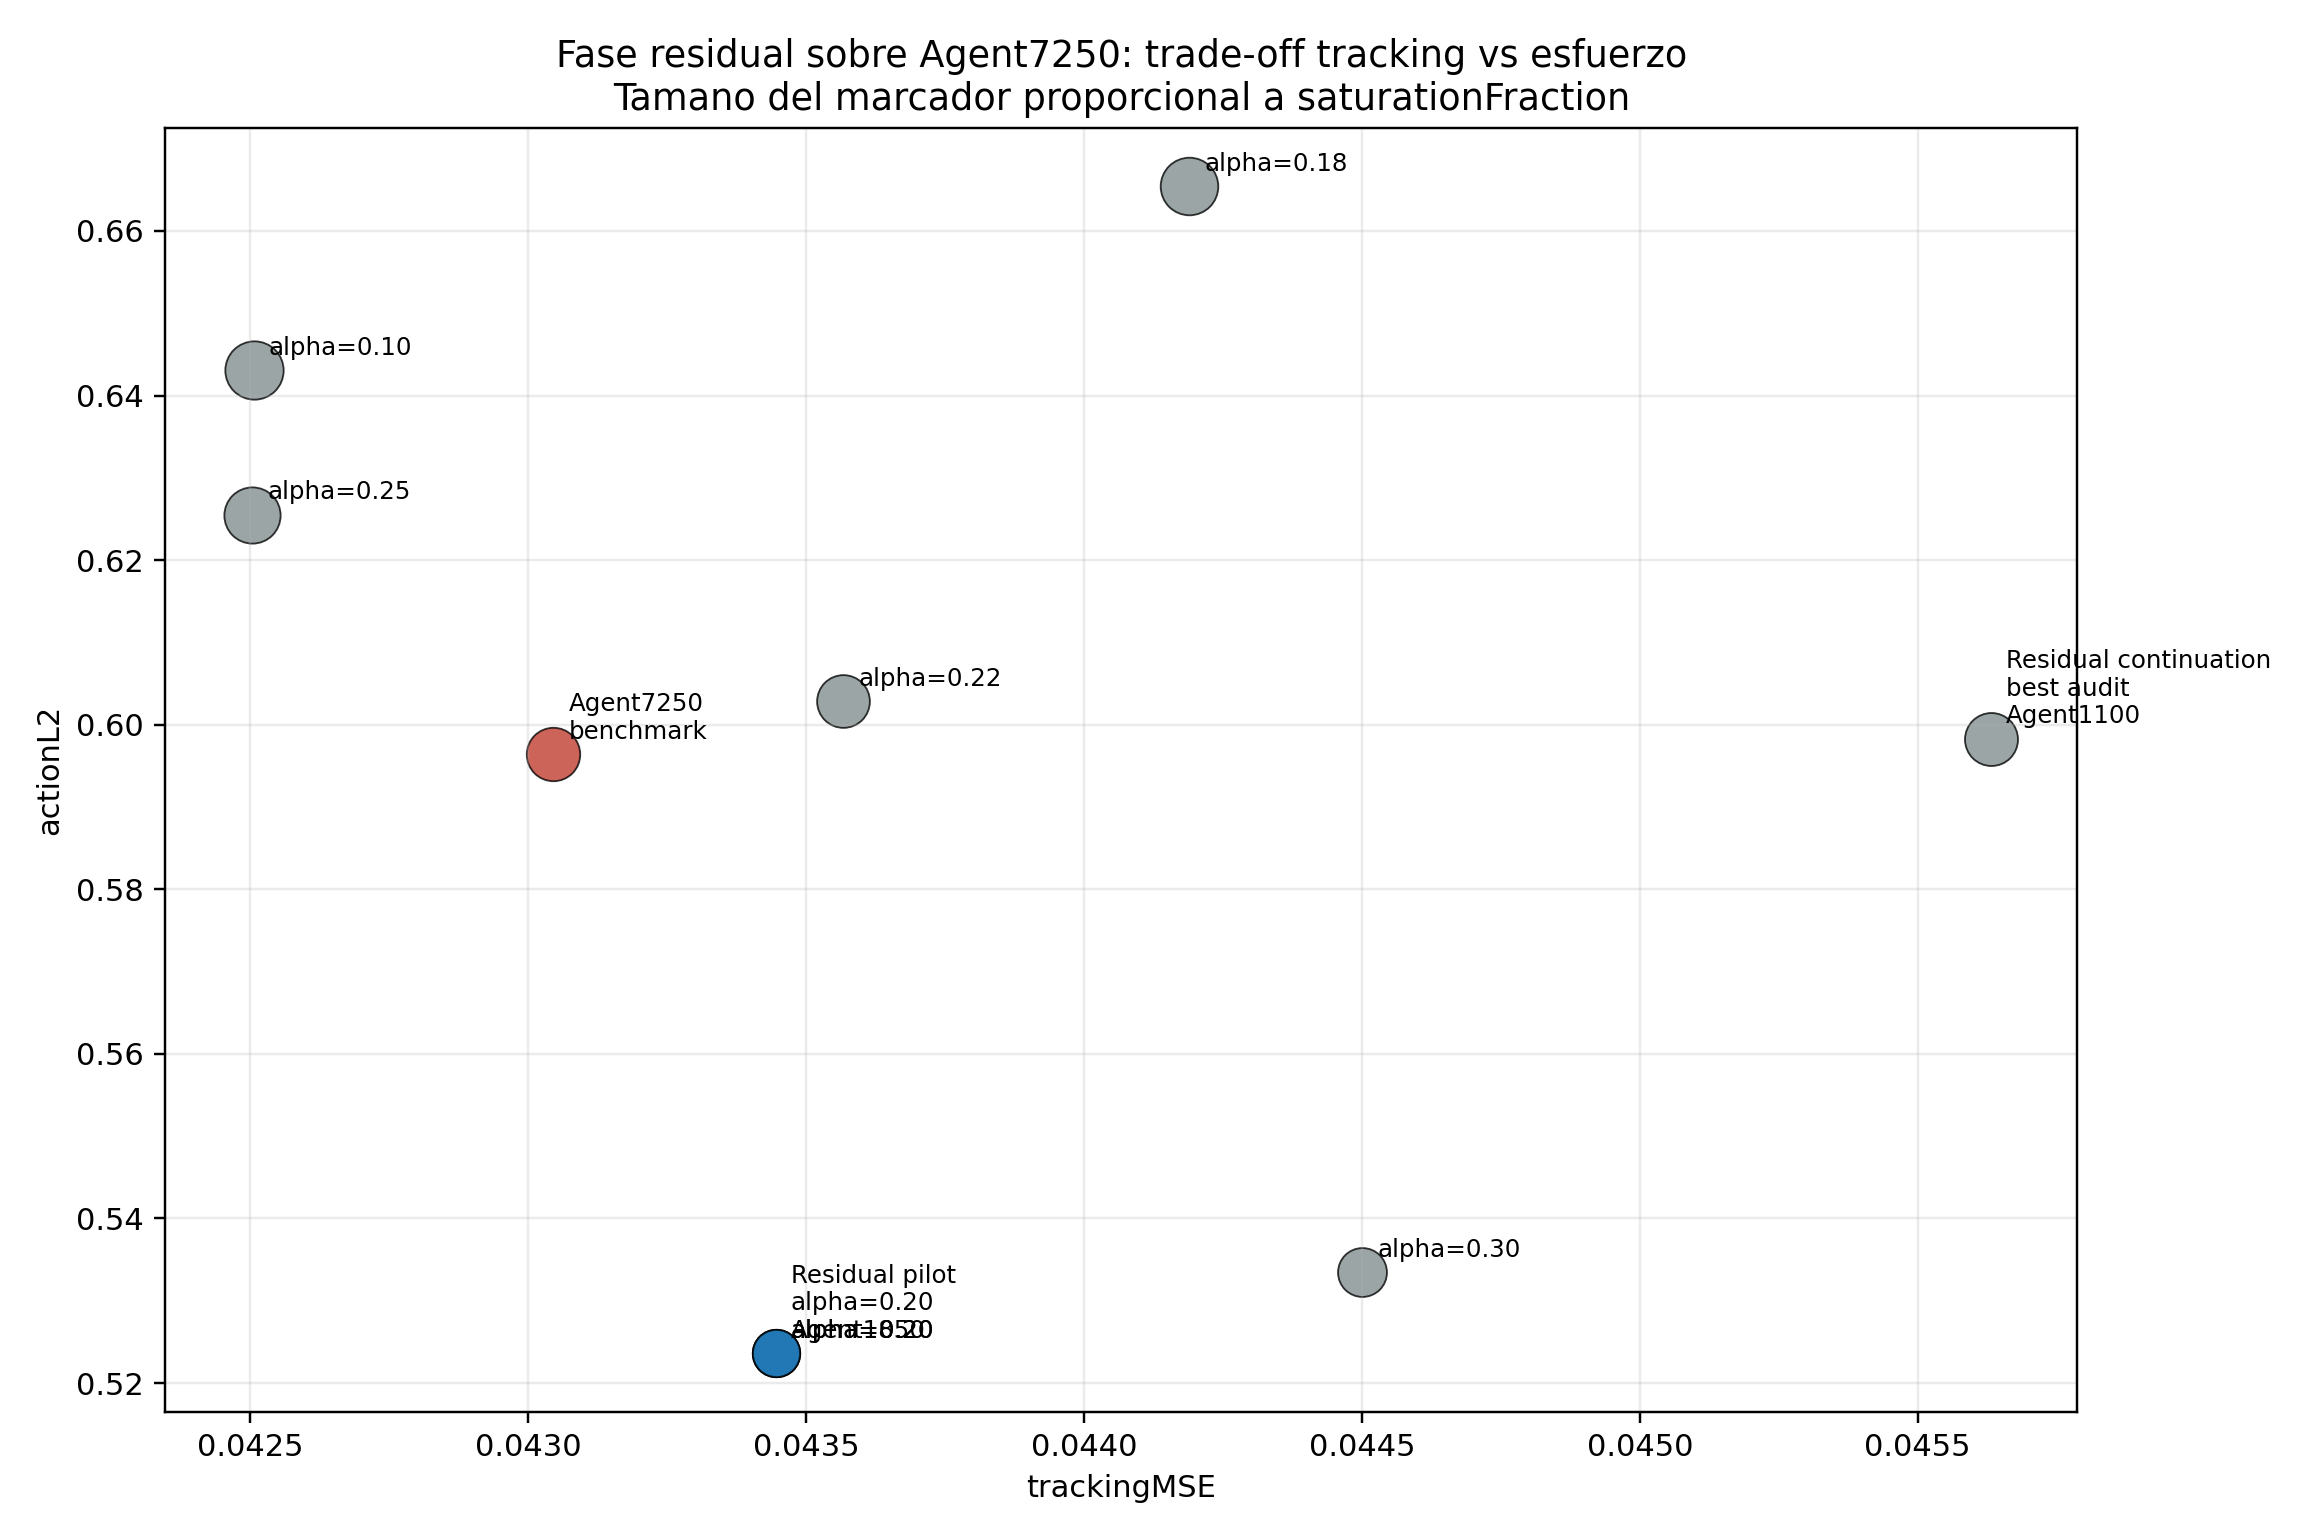
\includegraphics[width=0.98\linewidth]{figures/residual_phase_tradeoff_20260326.png}
\caption{Panorama completo de la fase residual. El mejor compromiso queda en la zona de \(\alpha_{\mathrm{res}} = 0.20\).}
\end{figure}

\subsection{Que dicen los diagnosticos residuales}

La fase residual no solo produjo una mejora; tambien dio una lectura mas rica del comportamiento del agente. En el mejor caso, la residual no colapso a una politica completamente nueva:
\begin{itemize}[leftmargin=1.5em]
\item \texttt{ResidualActionL2Mean} fue moderada;
\item \texttt{BaseToFinalActionDeltaMean} quedo contenida;
\item \texttt{SignOverrideFractionMean} fue baja.
\end{itemize}

Eso es importante porque indica que la mejora no vino de romper a la base, sino de corregirla de forma local y controlada. Esa es exactamente la logica que hace atractiva la familia residual \citep{silver2018residual,schaff2020shared,resfit2025}.

\begin{figure}[H]
\centering
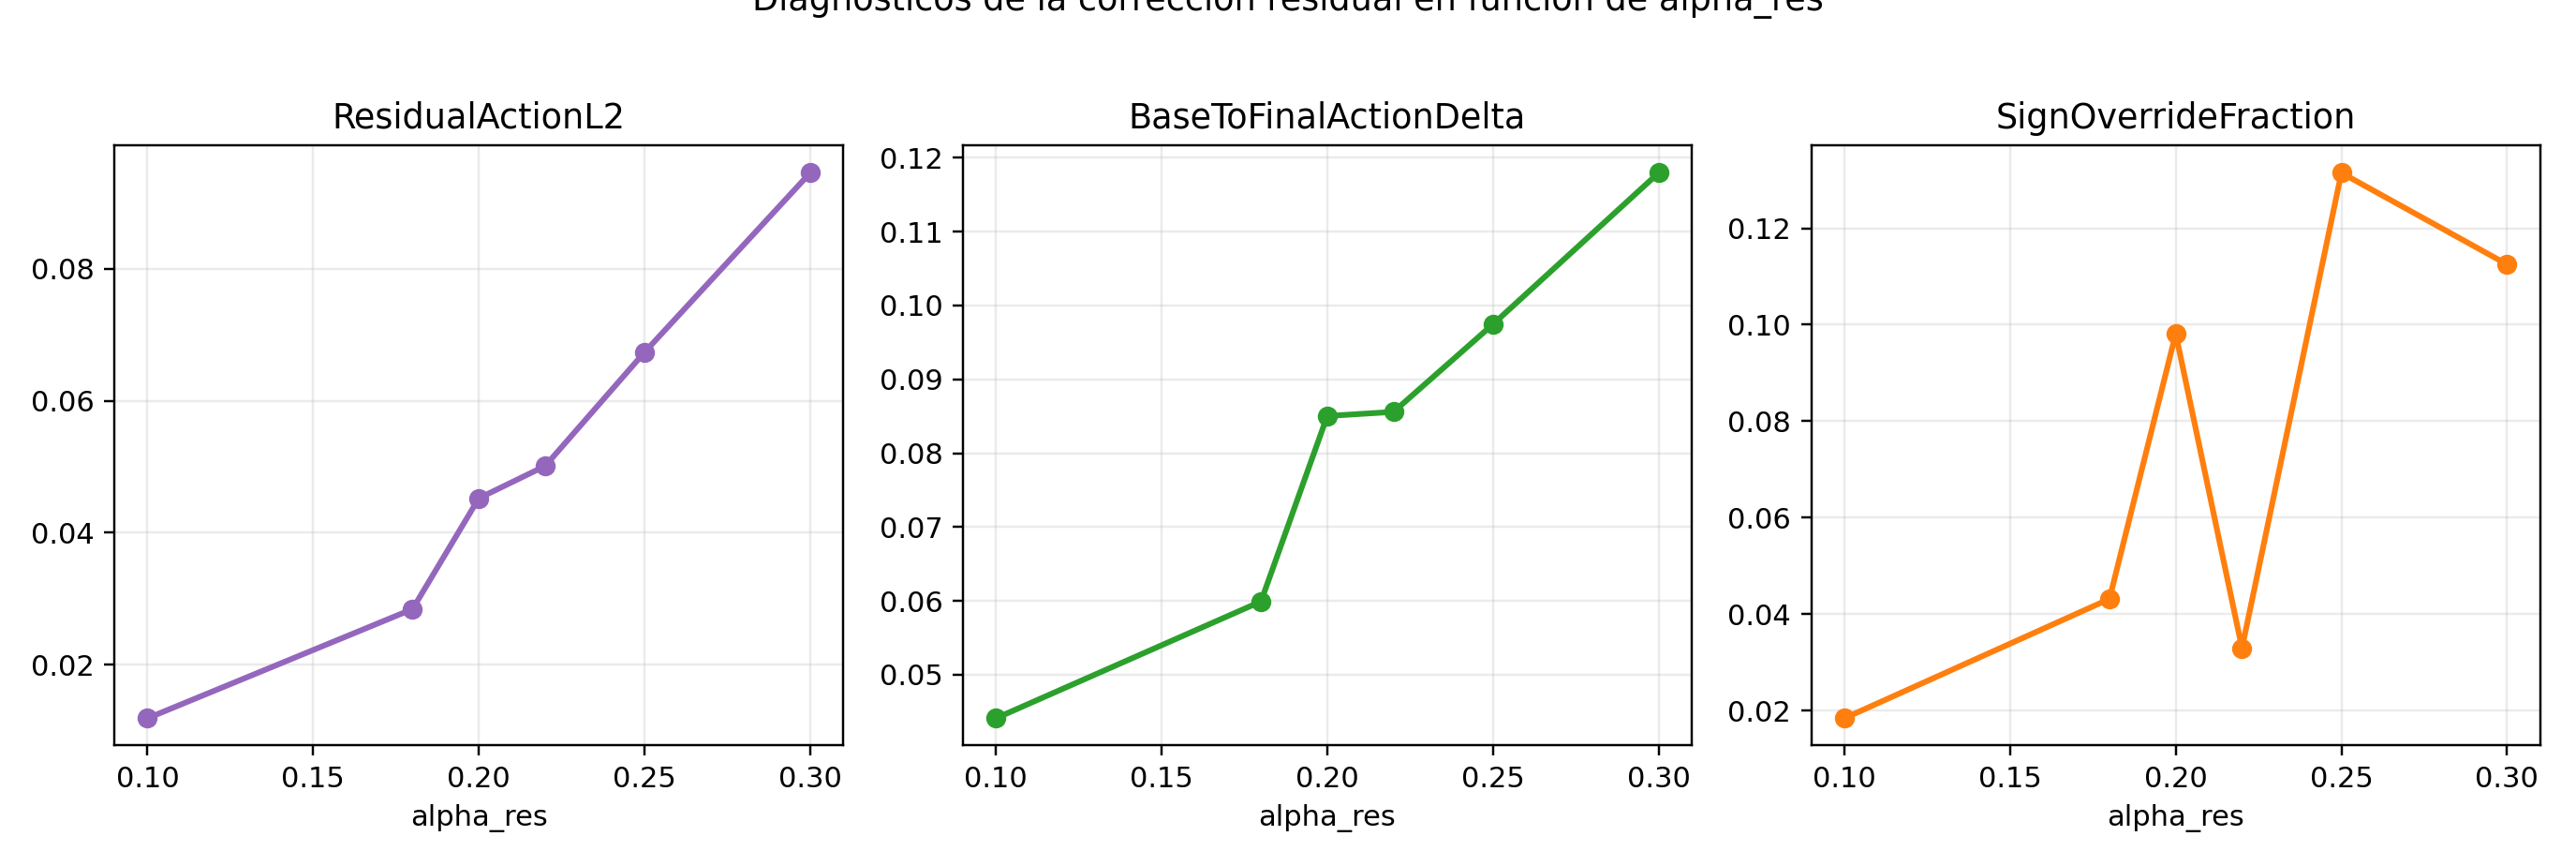
\includegraphics[width=0.96\linewidth]{figures/residual_alpha_diagnostics_20260326.png}
\caption{Diagnosticos de cuanto se aparta la politica residual respecto a la base. La zona de \(\alpha = 0.20\) mantiene una correccion moderada y util.}
\end{figure}

\section{Agente final recomendado}

Con la evidencia completa, el agente final recomendado por esta linea es:
\begin{itemize}[leftmargin=1.5em]
\item base historica congelada: \texttt{Agent7250},
\item mejor mejora encontrada: residual \texttt{Agent1850} con \(\alpha_{\mathrm{res}} = 0.20\).
\end{itemize}

La razon tecnica es directa:
\begin{itemize}[leftmargin=1.5em]
\item mantiene practicamente el tracking del benchmark;
\item reduce de forma clara saturacion y esfuerzo;
\item supera al benchmark bajo \texttt{ConditionB};
\item resistio tanto la continuacion como los barridos de \(\alpha\).
\end{itemize}

\section{Conclusion final}

La linea del proyecto puede resumirse asi:
\begin{enumerate}[leftmargin=1.5em]
\item el articulo base justifico TD3 y el control continuo;
\item el repositorio tuvo que depurar reward, accion efectiva y simulador antes de disponer de un benchmark valido;
\item la corrida post-fix de 8000 episodios produjo a \texttt{Agent7250} como benchmark serio;
\item las lineas posteriores a \texttt{Agent7250} exploraron varias rutas para bajar agresividad sin perder tracking;
\item la unica ruta que produjo una mejora defendible fue Residual TD3;
\item el punto final operativo de esa linea es el residual \texttt{Agent1850} con \(\alpha_{\mathrm{res}}=0.20\).
\end{enumerate}

Por tanto, si el proyecto necesita un cierre tecnico claro, la conclusion ya no es solo historica sino operativa:

\begin{quote}
el mejor candidato final del proyecto no es el benchmark base \texttt{Agent7250}, sino su mejora residual \texttt{Agent1850}, obtenida manteniendo la misma observacion, la misma reward y la misma logica de actuacion, pero aprendiendo una correccion pequena y bien regulada sobre la politica base.
\end{quote}

\bibliographystyle{unsrt}
\bibliography{references}

\end{document}
